\documentclass{article} % For LaTeX2e
\usepackage{nips15submit_e,times}
\usepackage[colorlinks,linkcolor=red]{hyperref}
\usepackage{url}
\usepackage{amsmath}
\usepackage{graphicx}
\usepackage{float}
\usepackage{bm}
\usepackage{amssymb}
%\documentstyle[nips14submit_09,times,art10]{article} % For LaTeX 2.09


\title{CS499 Homework 6 (First Draft)}


\author{
	Intersteller\thanks{ Use footnote for providing further information
		about author (webpage, alternative address)---\emph{not} for acknowledging
		funding agencies.}
	Department of Computer Science
	Cranberry-Lemon University
	Pittsburgh, PA 15213
}

% The \author macro works with any number of authors. There are two commands
% used to separate the names and addresses of multiple authors: \And and \AND.
%
% Using \And between authors leaves it to \LaTeX{} to determine where to break
% the lines. Using \AND forces a linebreak at that point. So, if \LaTeX{}
% puts 3 of 4 authors names on the first line, and the last on the second
% line, try using \AND instead of \And before the third author name.

\newcommand{\fix}{\marginpar{FIX}}
\newcommand{\new}{\marginpar{NEW}}

%\nipsfinalcopy % Uncomment for camera-ready version

\begin{document}

	\maketitle
	\textbf{Exercise 6.1}\par
	
	\textbf{Exercise 6.5}\par
	For every $n\le6$, there is an asymmetric graph on $n$ vertices, like Figure $1$.
  	\begin{figure}[H]
  	\centering
  	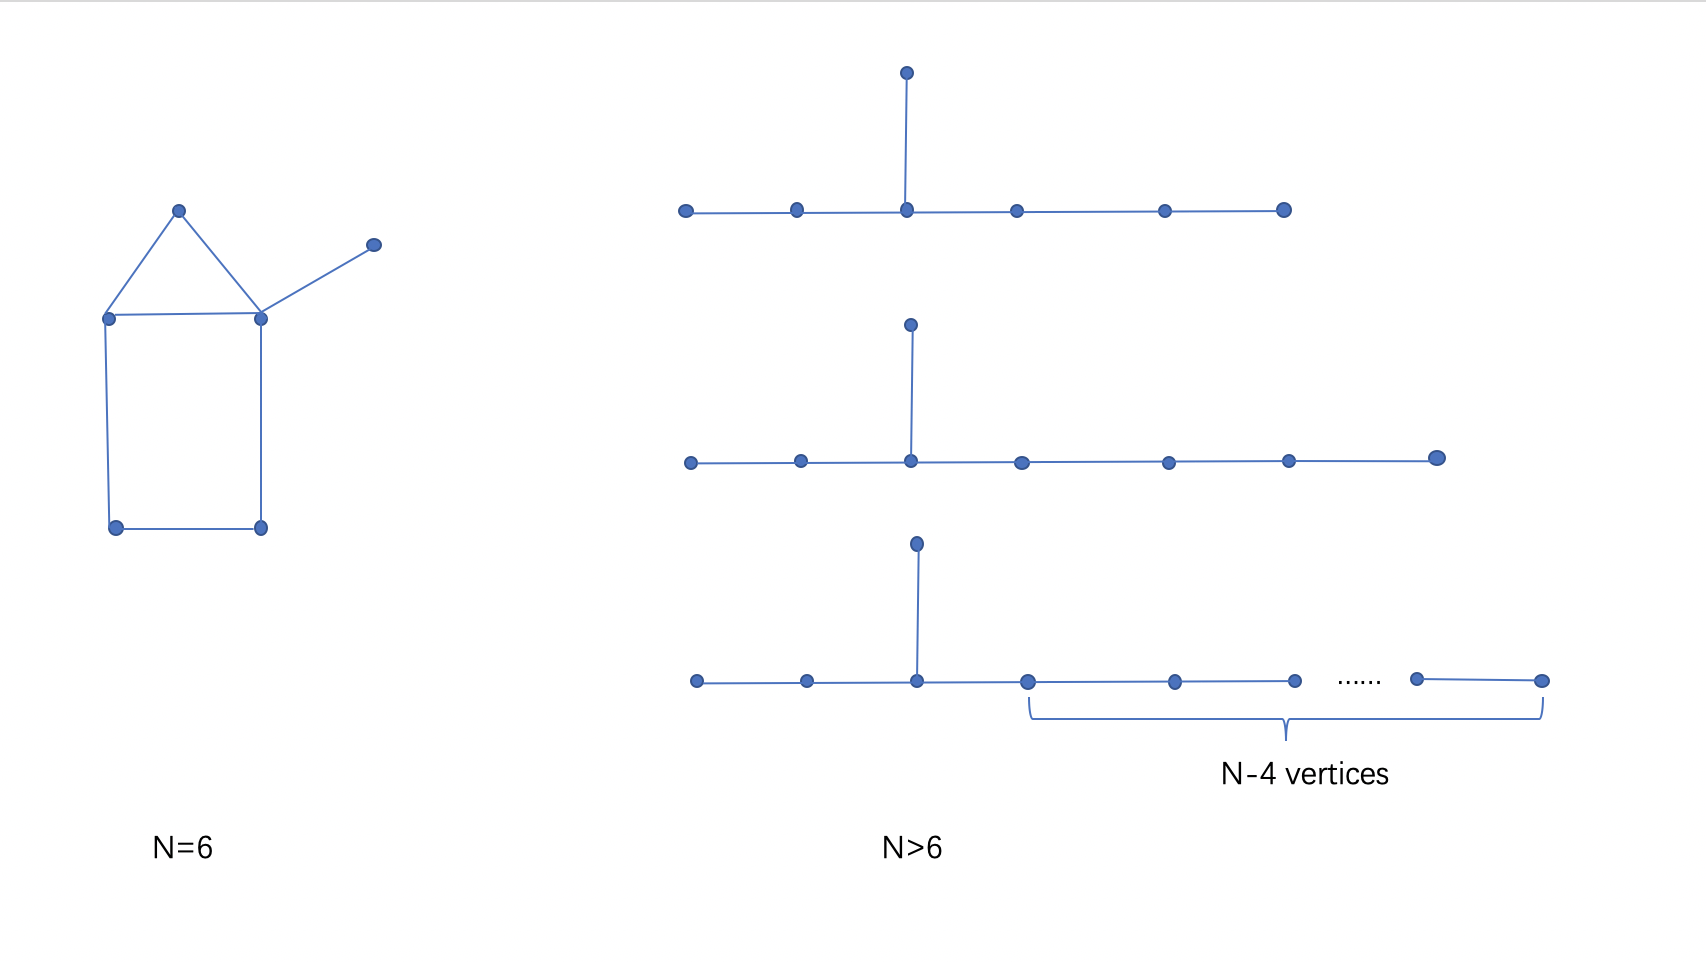
\includegraphics[scale=0.4]{6.5.png}
  	\caption{}
  	\label{fig:1}
  	\end{figure}
	When $n=6$, the left graph is correct. When $n>6$, we just need to construct trees like right graphs. 
	There are only one vertex that has three degrees and  $n-4$ vertices are at the right of this vertex.
	 
	\textbf{Exercise 6.6}\par
	For graphs in \textbf{Exercise 6.5}, we just need to add cherries for every vertex, like Figure $2$.
	\begin{figure}[H]
  	\centering
  	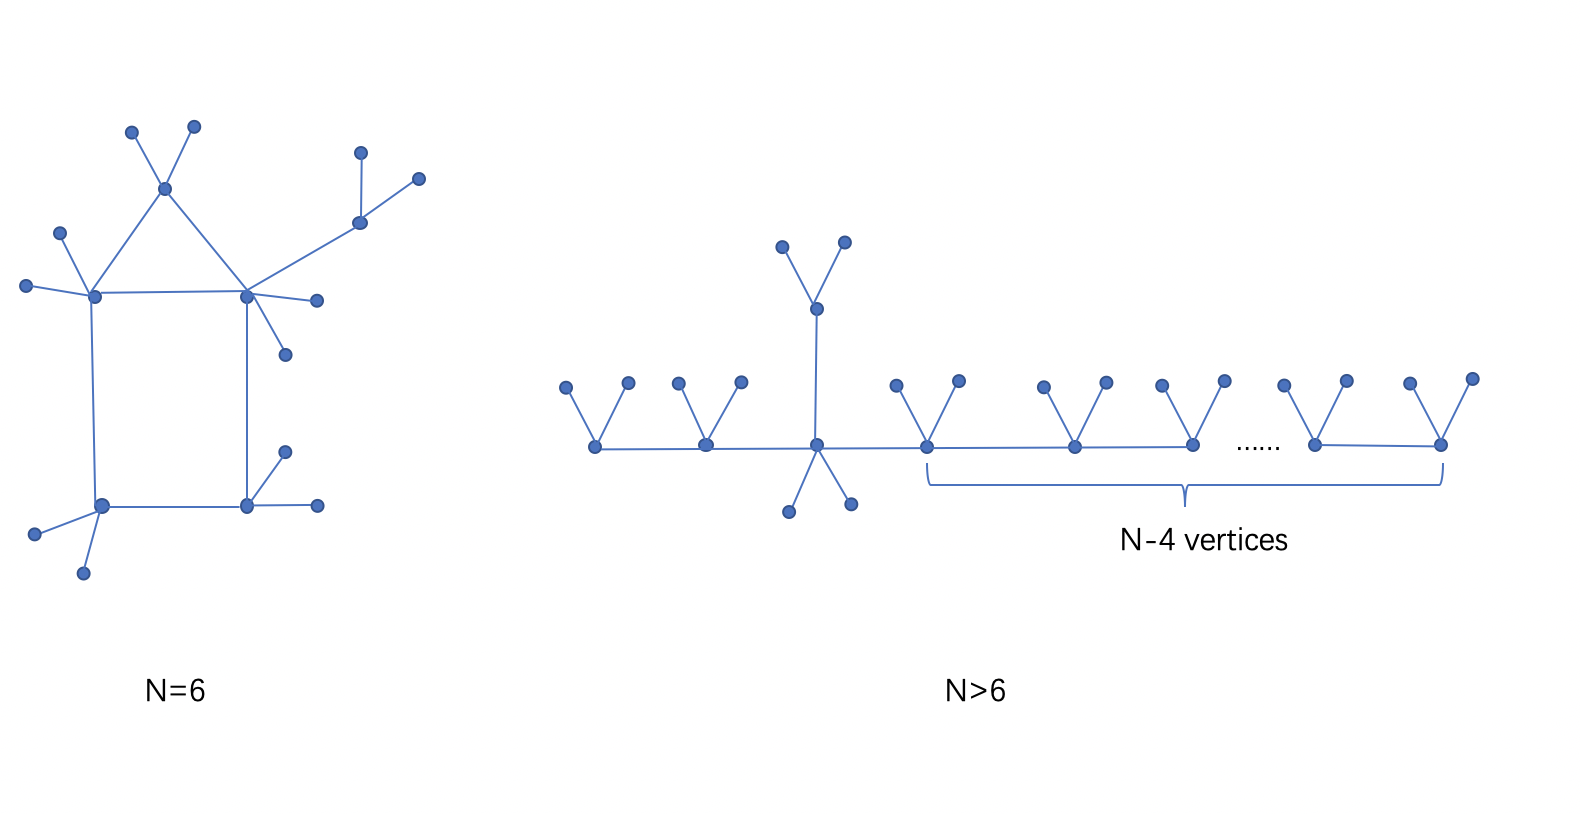
\includegraphics[scale=0.4]{6.6.png}
  	\caption{}
  	\label{fig:1}
  	\end{figure}
	The graph has $3n$ vertices with $2^{n}$ automorphisms.



	\textbf{Questions}\par
	

\end{document}
	

